\begin{figure}[htb]
	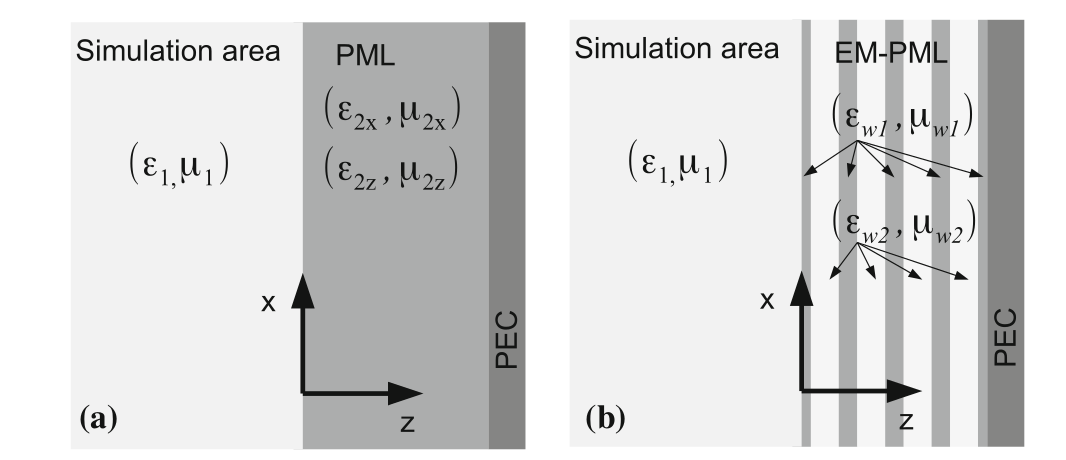
\includegraphics[width=\textwidth]{images/pml/oqe_schemat.png}
	\caption{Schematyczne przedstawienie analizowanej struktury warstwowej i~przybliżanego za pomocą modelu ośrodka efektywnego ośrodka PML}
	\label{fig:pml-multilay-schem}
\end{figure}

\subsection{Analityczne sformułowanie problemu}
Porównując ogólną postać PML podaną w~równaniu (\ref{eq:general-pml-form}) z~modelem ośrodka efektywnego przedstawionym w~podrozdziale \ref{subart:effmedium}, można zaproponować przybliżenie ośrodka typu PML za pomocą struktury warstwowej o~odpowiednich właściwościach efektywnych~\cite{ania2015}. Schematycznie taką wielowarstwę przedstawia rysunek \ref{fig:pml-multilay-schem}. W~szczególności, dla uproszczenia analizy, skupimy się na polaryzacji TM, dla której istotnymi składowymi tensorów opisujących własności materiałowe są:~$\varepsilon_x$~,$\mu_y$~i $\varepsilon_z$. Ze względu na ograniczenia używanego modelu ośrodka efektywnego, zgodnie ze schematem na rysunku \ref{fig:pml-multilay-schem} otrzymujemy $\varepsilon_x=\varepsilon_y$ oraz $\mu_x=\mu_y$. Ponownie odwołując się do granicy między ośrodkami na rysunku \ref{fig:pml-multilay-schem}a, otrzymujemy warunki, dla których wielowarstwa złożona z~materiałów $w1$ i~$w2$ schematycznie przedstawiona na rysunku \ref{fig:pml-multilay-schem}b, będzie efektywnie spełniać rolę PML pod warunkiem spełnienia następujących równości:
\begin{equation}
	f\cdot \varepsilon_{w1} + (1-f)\cdot \varepsilon_{w2} = s \cdot \varepsilon_1,
	\label{eq:oqe4}
\end{equation}

\begin{equation}
	[f\cdot \varepsilon_{w1}^{-1}+(1-f)\varepsilon_{w2}^{-1}]^{-1}=s^{-1}\cdot \varepsilon_1,
	\label{eq:oqe5}
\end{equation}

\begin{equation}
	f\cdot \mu_{w1} + (1-f)\cdot \mu_{w2} = s \cdot \mu_1,
	\label{eq:oqe6}
\end{equation}
gdzie przez $f$ oznaczony został współczynnik wypełnienia, równy ułamkowi przestrzeni wielowarstwy zajmowanemu przez materiał $w1$. Odpowiednie warunki dla polaryzacji TM to:
\begin{equation}
	\varepsilon_{w1}=\rho \frac{\varepsilon_1 \cdot s}{f\cdot \rho + (1 -f) },
	\label{eq:te-eps1}
\end{equation}

\begin{equation}
	\varepsilon_{w2}=\frac{\varepsilon_1 \cdot s}{f\cdot \rho + (1-f)},
	\label{eq:te-eps2}
\end{equation}
gdzie
\begin{equation}
	\rho = 1+\frac{s^2-1 \pm \sqrt{(s^2-1)(s^2-(2f-1)^2)}}{2f(1-f)}.
	\label{eq:te-rho}
\end{equation}

\begin{figure}[htb]
	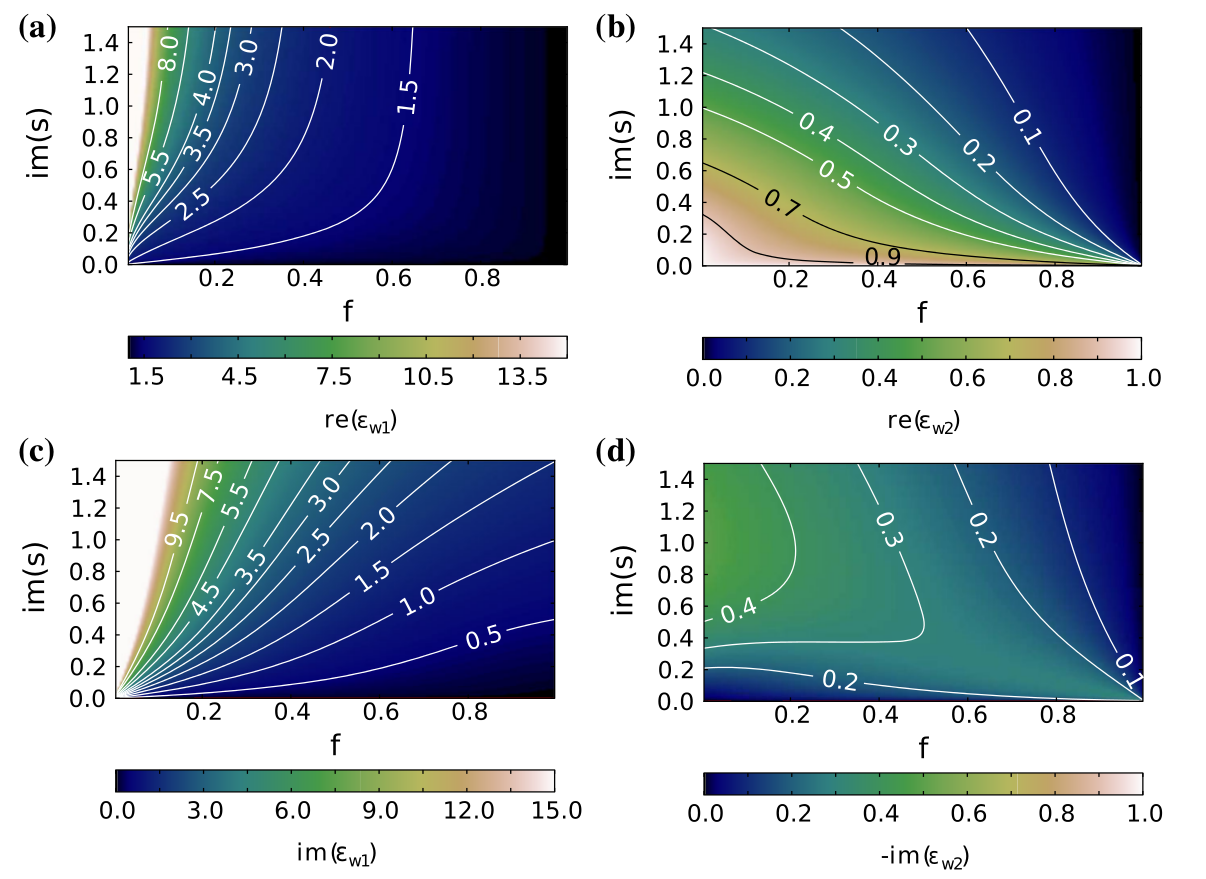
\includegraphics[width=\textwidth]{images/pml/oqe_materials.png}
	\caption{Zależność przenikalności elektrycznej materiałów tworzących UPML (w lewej kolumnie $\varepsilon_{w1}$, w~prawej $\varepsilon_{w2}$) w~funkcji współczynnika wypełnienia i~urojonej części parametru $s$ (założono, że $\textrm{Re}(s)$=1. Górny wiersz na wykresach (a) i~(b) prezentuje zależności części rzeczywistych, dolny na wykresach (c) i~(d) części urojonych przenikalności elektrycznych. Ujemne wartości $\varepsilon$ na wykresach (c) i~(d) odpowiadają materiałom ze wzmocnieniem optycznym~\cite{ania2015}. }
	\label{fig:upml-eps-s-f}
\end{figure}

Wykresy na rysunku \ref{fig:upml-eps-s-f} prezentują wyniki obliczonych zgodnie z~(\ref{eq:te-eps1}) i~(\ref{eq:te-eps2}) wartości $\varepsilon_{w1}$ i~$\varepsilon_{w2}$ jako funkcje współczynnika wypełnienia $f$ i~parametru $s$, dla którego przyjęto $s=1+\alpha i$. Używamy rozwiązań dla (\ref{eq:te-rho}) z~$|\rho|>1$. Podobne wyrażenia jak (\ref{eq:oqe4}) i~(\ref{eq:oqe5}) można wypisać i~rozwiązać dla $\mu_{w1}$ i~$\mu_{w2}$. W przypadku gdy $\varepsilon_1=\mu_1$ otrzymujemy $\varepsilon_{w1}=\mu_{w1}$ i~$\varepsilon_{w2}=\mu_{w2}$. Należy podkreślić, że dla każdej pary $f$ i~$s$ przedstawionej na wykresach \ref{fig:upml-eps-s-f} uzyskujemy metamateriał, który w~omawianym przybliżeniu będzie spełniał funkcje UPML. Dla każdej pary $f$ i~$s$ potrzebujemy jednak wybrać inne materiały $w1$ i~$w2$.

W kolejnym kroku możemy obliczyć natężeniowy współczynnik odbicia od struktury zaprezentowanej na rysunku \ref{fig:pml-multilay-schem}b dla $f=0.6$ oraz $\textrm{Im}(s)=$0.5 lub $\textrm{Im}(s)=$5. Zależność współczynnika odbicia od kąta padania oraz grubości komórki elementarnej wielowarstwy przedstawia wykres na rysunku \ref{fig:oqe3}. Ze względu na umieszczenie idealnego przewodnika za wielowarstwą, współczynnik odbicia łączy w~sobie część odbijaną od wielowarstwy, jak i~transmitowaną przez wielowarstwę i~odbijaną od zwierciadła z~PEC~(ang. perfect electric conductor) . Analizując wykres \ref{fig:oqe3}, możemy zauważyć, że wraz ze wzrostem $\frac{a}{\lambda}$ zmniejsza się współczynnik odbicia fal propagujących się, którym odpowiada część wykresu, dla którego na osi odciętych wartości spełniają nierówność $\frac{k_x}{k_0}<1$.

Wynika to ze zwiększania grubości warstwy pochłaniającej, więc jest przede wszystkim związane ze zmniejszeniem transmisji przez wielowarstwę, a nie zmianą odbicia od pierwszej granicy warstw. W przypadku fal ewanescentnych $\frac{k_x}{k_0}>1$ obserwujemy wzrost współczynnika odbicia. Można to interpretować jako zwiększenie odbicia od pierwszej warstwy wynikające z~niespełnienia warunków homogenizacji (przybliżenie ośrodka efektywnego zakłada $\frac{a}{\lambda} <<$ 1) przez strukturę. Dlatego wzrost jest większy dla większej części urojonej współczynnika $s$, skutkującej większą różnicą współczynników załamania na granicy pierwszej warstwy i~powietrza.

\begin{figure}[htb]
	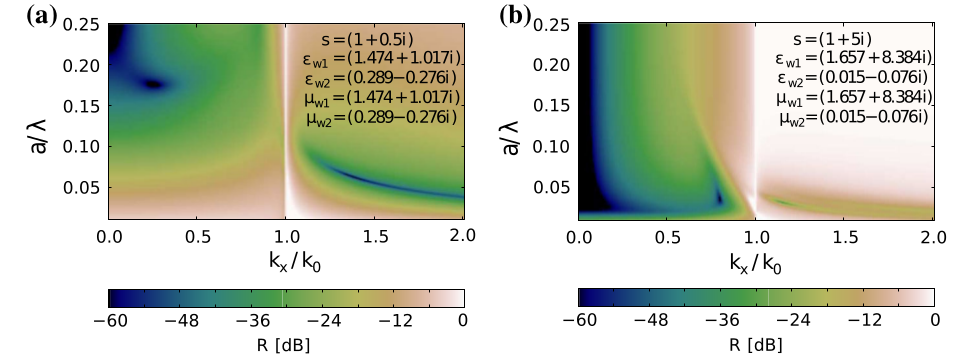
\includegraphics[width=\textwidth]{images/pml/fig3.png}
	\caption{Zależność natężeniowego współczynnika odbicia od kąta padania i~okresu wielowarstwy dla struktury zgodniej ze schematem na rysunku \ref{fig:pml-multilay-schem}, dla $N=5$ par warstw, przy współczynniku wypełnienia $f=0.6$. Rysunek po lewej (a) przedstawia wyniki dla $s=1+0.5i$, wykres po prawej(b) przedstawia wyniki dla $s=1+5i$. Przez $a$ oznaczono rozmiar komórki elementarnej wielowarstwy~\cite{ania2015}.}
	\label{fig:oqe3}
\end{figure}

Przedstawione wyniki możliwe są do osiągnięcia za pomocą materiałów wykazujących szczególne własności elektryczne i~magnetyczne. W szczególności obliczenia zakładały zespoloną przenikalność magnetyczną oraz wzmocnienie optyczne. Dla $s=1+5i$ możliwe jest uzyskanie warstwy PML o~całkowitej grubości $5\cdot a \approx \frac{\lambda}{20}$ wykazującej natężeniowy współczynnik odbicia ok -30dB dla szerokiego zakresu kątów padających fal płaskich.

W przypadku oświetlenia wielowarstwy za pomocą fali o~polaryzacji TM, jeden ze współczynników przenikalności magnetycznej może zostać ustalony w~sposób arbitralny. W szczególności możemy więc założyć $\mu_{w2}=1$, ponieważ większość materiałów spotykanych w~przyrodzie charakteryzuje się taką wartością dla częstotliwości optycznych. Drugą przenikalność magnetyczną możemy wyznaczyć za pomocą wzoru (\ref{eq:oqe6}). Część rzeczywista $\textrm{Re}(\mu_{w1})=1$, a zależność części urojonej $\textrm{Im}(\mu_{w1})$ od części urojonej współczynnika $s$ oraz współczynnika wypełnienia $f$ przedstawia wykres \ref{fig:im-mu1}. Na podstawie przywołanego wykresu możemy zauważyć, że wysoki współczynnik wypełnienia oraz wykorzystanie niskiej części urojonej $s$ skutkują niskimi wartościami $\textrm{Im}(\mu_{w1})$. Jest to dla nas istotne, ponieważ korzystając z~materiałów występujących w naturze, będziemy zmuszeni przybliżyć tę wartość przez $0$.

\begin{SCfigure}
	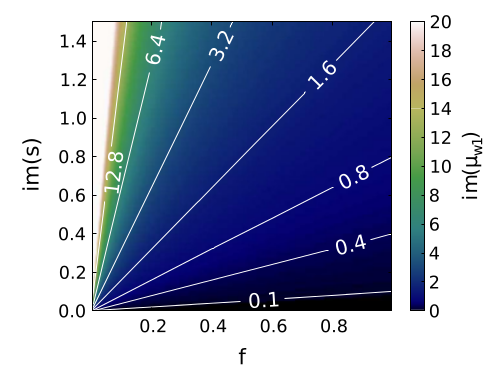
\includegraphics[width=0.6\textwidth]{images/pml/fig4.png}
	\caption{Zależność części urojonej przenikalności magnetycznej jednego z~materiałów $\mu_{w1}$, od części urojonej współczynnika $s$ i~współczynnika wypełnienia $f$ w~przypadku, gdy założono $\mu_{w2}=1$~\cite{ania2015}}
	\label{fig:im-mu1}
\end{SCfigure}

\subsection{Wykorzystanie materiałów występujących w przyrodzie}

W przypadku przygotowania eksperymentu, a nie np. wykorzystania do konstrukcji PML w~symulacjach  numerycznych, należy zaniedbać nie tylko własności magnetyczne materiałów $\mu=1$, ale również zysk optyczny $\textrm{Im}(\varepsilon)<0$~\footnote{Istniejące w przyrodzie materiały dla zakresu optycznego i podczerwieni charakteryzują się $\mu \approx 1$ i nie posiadają wzmocnienia}. Wyniki dla obu polaryzacji po zastosowaniu się do wymienionych ograniczeń przedstawiają wykresy na rysunku \ref{fig:pml-real-ref}. Zaproponowany absorber składa się z~materiału stratnego oraz warstw charakteryzujących się przenikalnością elektryczną mniejszą od 1. Przedstawione wyniki obliczeń wskazują, że w~wyniku poczynionych założeń efektywność pracy wielowarstwy jako struktury PML znacznie różni się w~zależności od polaryzacji. W przeciwieństwie do obliczeń dla wielowarstw odpowiadających PML, narzucone warunki prowadzą do mniejszej wartości współczynnika odbicia dla polaryzacji TE. Wysokie współczynniki odbicia, uniemożliwiające zastosowanie wielowarstwy,  pojawiają się jednak jedynie dla kątów padania bliskich $90^{\circ}$, co jest charakterystyczne dla UPML.

\begin{figure}[htb]
	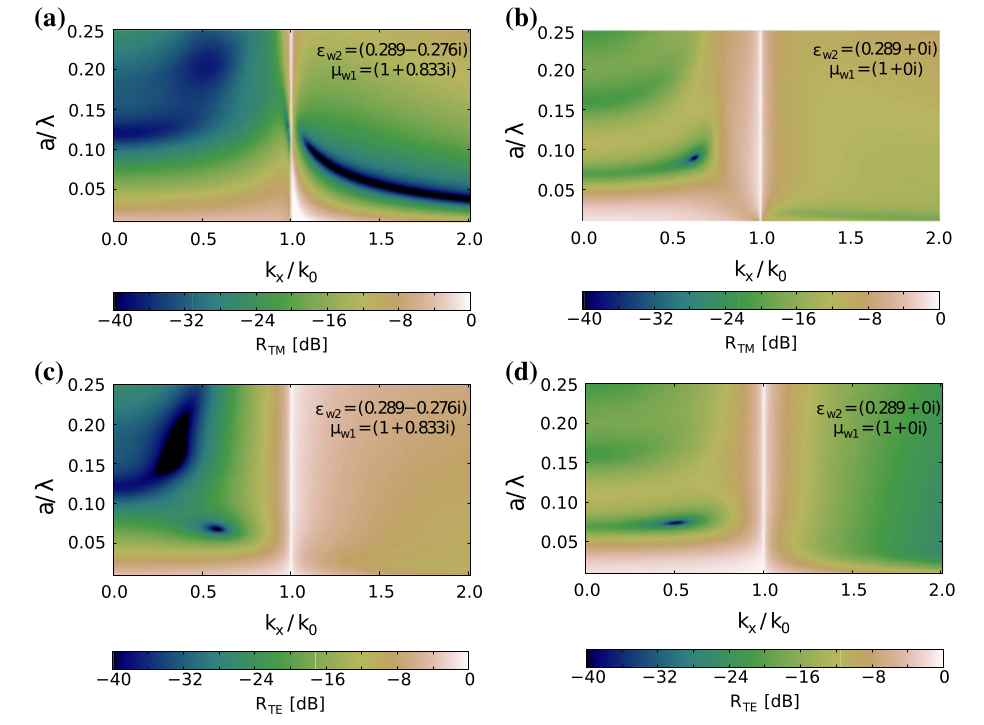
\includegraphics[width=\textwidth]{images/pml/fig5.png}
	\caption{Zależność natężeniowego współczynnika odbicia $R$, od kąta padania i~grubości warstw dla wielowarstwy składającej się z~$N=5$ okresów, dla $s=1+5i$ i~$f=0.6$. Spełniając założenie, że $\mu_{w2}=1$ (a,c) oraz $\mu_{w1}=\mu_{w2}=1$, $\textrm{Im}(\varepsilon_1)\ge 0 $ i~$\textrm{Im}(\varepsilon_2)\ge 0 $ (b,d). Wyniki dla polaryzacji TM (a,b) oraz TE (c,d). Przenikalność elektryczna $\varepsilon_{w1}=1.474+1.017i$~\cite{ania2015}.}
	\label{fig:pml-real-ref}
\end{figure}


Na podstawie przeprowadzonej dyskusji, można zaproponować prostą regułę jaką należy posługiwać się w~celu doboru materiałów do budowy wielowarstwy efektywnie przypominającej UPML na granicy z~powietrzem. Kluczowym elementem jest wykorzystanie materiału, którego część rzeczywista przenikalności elektrycznej znajduje się w~zakresie od 0 do 1. Przeprowadzone obliczenia wskazują również, że materiał ten powinien być możliwe bezstratny. Druga wykorzystywana substancja powinna posiadać część rzeczywistą przenikalności elektrycznej większą od~1, jak i~wykazywać stratność. 

W ogólności w~szerokich zakresach spektralnych większość materiałów charakteryzuje się $\textrm{Re}(\varepsilon) > 1$. Wyjątkami są zakresy długości fali w~okolicach rezonansów dyspersyjnych (patrz. \ref{subart:lorenz-drude}). Możliwe jest również uzyskanie zaprojektowanych własności $\varepsilon$ w~metamateriałach np. w~strukturach funkcjonujących w~literaturze angielskojęzycznej pod nazwą \textit{fishnet}~\cite{valentine2008three}. 

Przykładem pary materiałów, które możemy zastosować w~realizacji UPML za pomocą wielowarstwy są $SiO_2$ i~$NaCl$ dla długości fali w~okolicach 8~µm. Przenikalności elektryczne zaproponowanych materiałów przedstawiają wykresy na rysunku \ref{fig:nacl-sio2-mat}. Rolę materiału o~przenikalności elektrycznej $\varepsilon \in (0,1)$, spełnia w~tym obszarze $SiO_2$, ponieważ dla długości fali $9.5$~µm występuje dla tego materiału rezonans. Również wartość efektywna części urojonej $\varepsilon$ wielowarstwy wynika głównie z~własności $SiO_2$. 

\begin{figure}[htb]
	\begin{subfigure}{0.45\textwidth}
		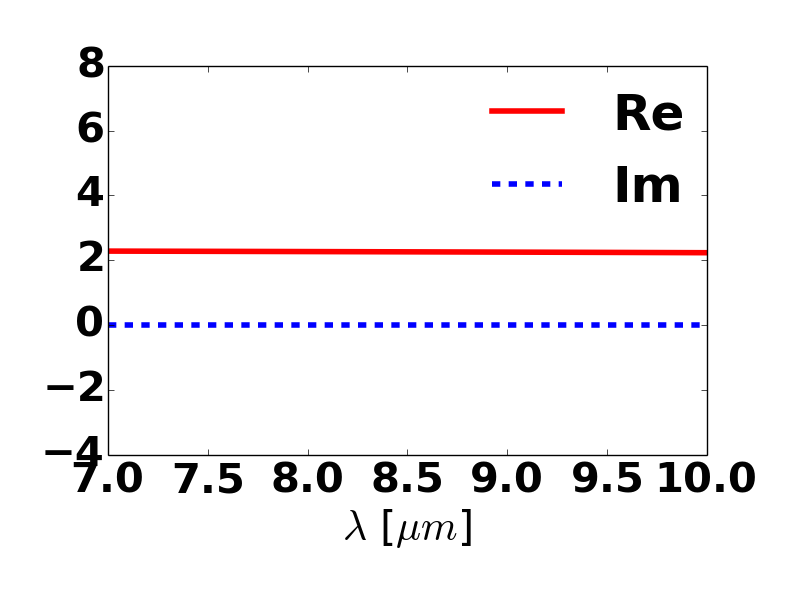
\includegraphics[width=\textwidth]{images/pml/nacl.png}
		\caption{}
	\end{subfigure}
	\begin{subfigure}{0.45\textwidth}
		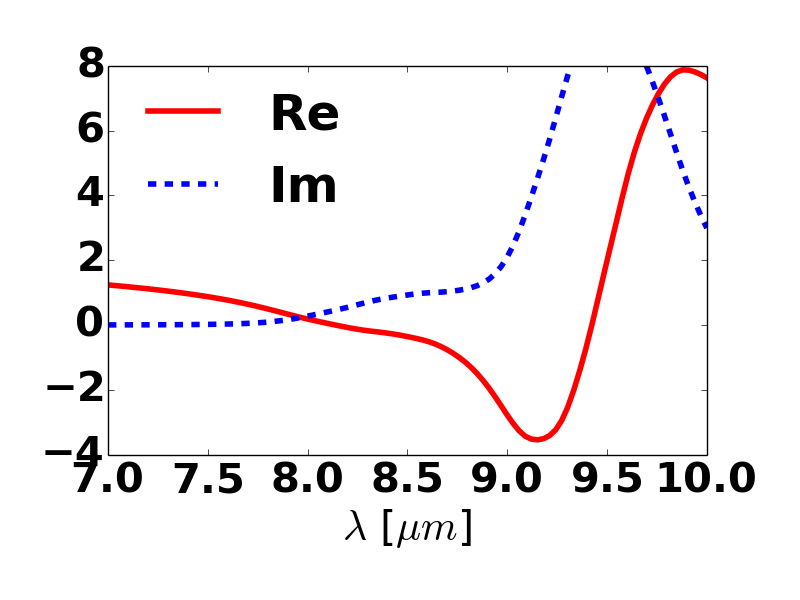
\includegraphics[width=\textwidth]{images/pml/sio2.png}	
		\caption{}
	\end{subfigure}
	\caption{Wartości przenikalności elektrycznej w~zakresie długości fali od 7 do 10~µm dla (a) $NaCl$~\cite{li1976refractive}, (b) $SiO_2$~\cite{Kischkat:12}}
	\label{fig:nacl-sio2-mat}
\end{figure}

Efektywne własności stosu złożonego z~naprzemiennych warstw $NaCl$ i~$SiO_2$ o~współczynniku wypełnienia drugim materiałem $f=0.56$, dla których przyjęto zmierzone eksperymentalnie wartości $\varepsilon$, przedstawia wykres na rysunku \ref{fig:eff-pml-real}. Zgodnie z~(\ref{eq:general-pml-form}) struktura warstwowa przypominająca PML powinna spełniać związek $\frac{1}{\varepsilon_x}=\varepsilon_z$, dlatego na wykresie zaznaczono również wartość $\frac{1}{\varepsilon_x}$. Na podstawie wykresu \ref{fig:eff-pml-real}, wielowarstwa powinna więc charakteryzować się najniższym współczynnikiem odbicia dla długości fali z~zakresu 8.0-8.2~µm. Wartości natężeniowych współczynników transmisji i~odbicia w~zależności od liczby par warstw $N$ oraz długości fali przedstawia wykres na rysunku \ref{fig:oqe-trans-refl}.

\begin{SCfigure}
	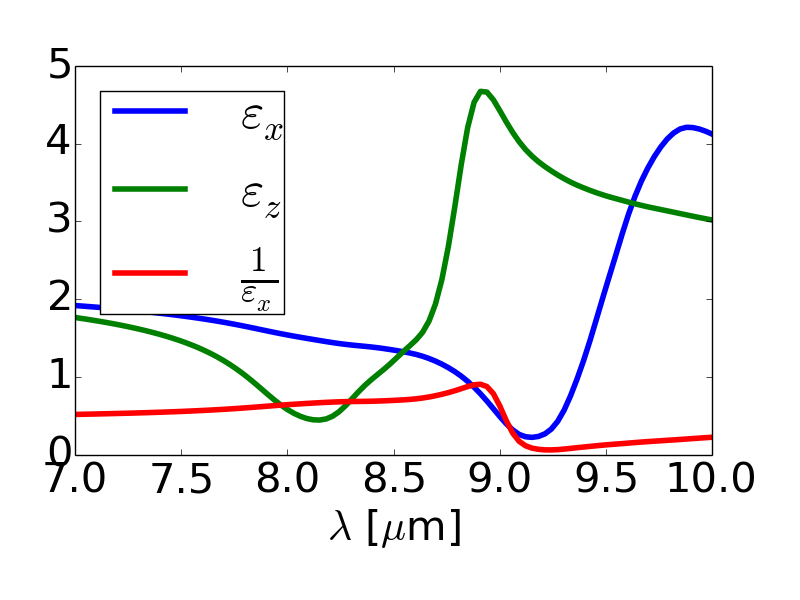
\includegraphics[width=0.6\textwidth]{images/pml/effepsilon-nacl-sio2.png}
	\caption{Składowe $\varepsilon_x$ i $\varepsilon_z$ efektywnego tensora przenikalności elektrycznej wielowarstwy zbudowanej z~$SiO_2$ i~$NaCl$, o~współczynniku wypełnienia przez $SiO_2$ równym $f=0.56$.}
	\label{fig:eff-pml-real}
\end{SCfigure}

Opierając się na zaprojektowanej wielowarstwie można zaproponować jej modyfikację w~geometrii cylindrycznej. W tym przypadku jakość nieodbijającej warstwy absorpcyjnej możemy ocenić na podstawie symulacji, w~których wewnątrz struktury typu \textit{core-shell} zamknięty zostanie walec z~idealnego przewodnika. Rozkład gęstości energii pola E-M dla struktury typu \textit{core-shell} odpowiadającej rozważanej wielowarstwie, oświetlonej falą monochromatyczną dla polaryzacji TM~i~TE przedstawia rysunek \ref{fig:oqecoreshell}.

\begin{figure}[htb]
	\centering
	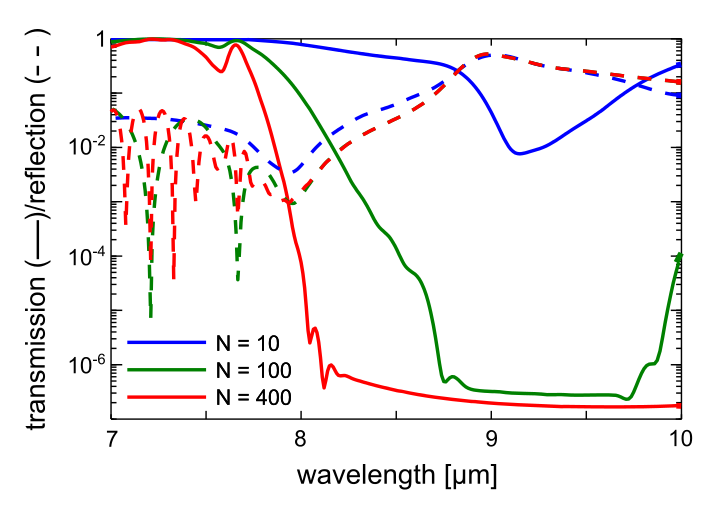
\includegraphics[width=0.6\textwidth]{images/pml/oqe_trans_refl.png}
	\caption{Współczynnik transmisji (linia ciągła) i~odbicia (linia przerywana) dla wielowarstwy złożonej z~$SiO_2$/$NaCl$ zaprojektowanej dla oświetlenia falą o długości 8~µm, dla której współczynniki załamania $n_{\textrm{SiO}_2}=0.41+0.32i$, $n_{\textrm{NaCl}}=$~1.51. Współczynnik wypełnienia struktury przez $SiO_2$ wynosi $f=0.56$, $a=200nm$. Rozważone zostały stosy o~liczbie par warstw $N=$~10,~100 i~400~\cite{ania2015}.}
	\label{fig:oqe-trans-refl}
\end{figure}

\begin{figure}[htb]
	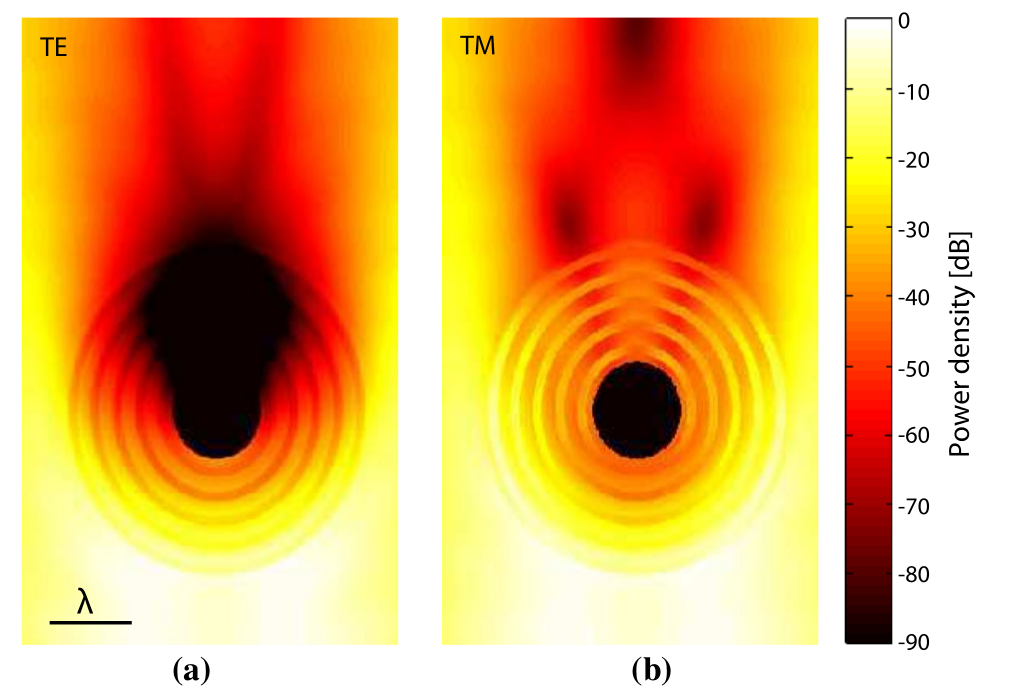
\includegraphics[width=\textwidth]{images/pml/oqe_coreshell.png}
	\caption{Wyniki symulacji w geometrii cylindrycznej dla polaryzacji (a) TE i~(b) TM. Struktura typu core-shell oświetlona jest z~dołu. Na rysunku (a) zamieszczono wzorzec długości fali.}
	\label{fig:oqecoreshell}
\end{figure}

\subsection{Podsumowanie wyników}

Porównując uzyskane wyniki do warstw absorbujących otrzymywanych innymi metodami, należy dosyć krytycznie ocenić możliwość wykorzystania tego typu struktur w zastosowaniach eksperymentalnych. Wprowadzone uproszczenia umożliwiły zaproponowanie fizycznej realizacji absorbera w oparciu o realne materiały, jednak wartości współczynnika odbicia, w szczególności dla dużych kątów padania, nie są satysfakcjonujące. Należy również zwrócić uwagę, że uzyskanie wysokiego współczynnika absorpcji jest możliwe przy zastosowaniu znaczącej liczby par warstw, w wyniku czego metamateriał tworzący warstwę absorpcyjną staje się znacznie grubszy od długości fali. 

\begin{figure}[htb]
	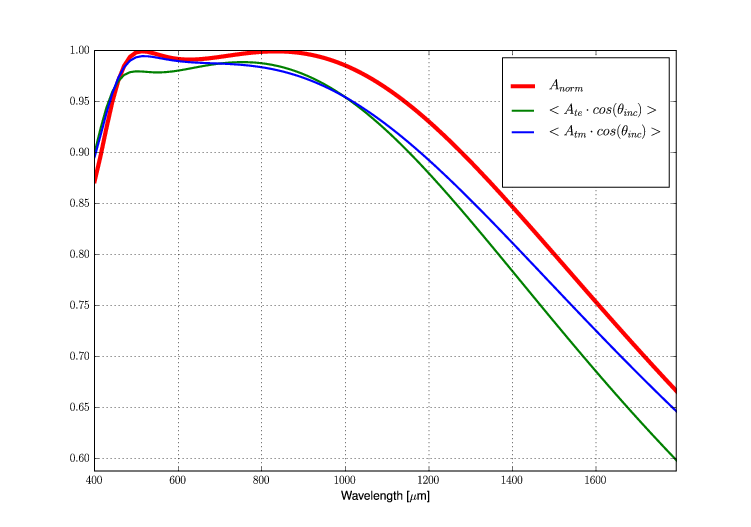
\includegraphics[width=0.8\textwidth]{images/pml/optiabsorb.png}
	\caption{Zależność współczynnika absorpcji od długości fali dla padania normalnego oraz uśrednionego po cosinusach kątów dla polaryzacji TM i TE dla zoptymalizowanej wielowarstwy $NiCr$-$BrF_2$~\cite{stefaniuk2015perfectly}}
	\label{fig:optimulti}
\end{figure}

Alternatywnie do problemu realizacji absorbera za pomocą struktury warstwowej można zastosować optymalizację parametrów - definiując jako kryterium maksymalizację liniowej kombinacji absorpcji przy padaniu światła pod kątem normalnym oraz uśrednionych ze względu na kąt padania absorpcji promieniowania padającego w polaryzacjach TM i TE~\cite{stefaniuk2015perfectly}. Wynik takiej optymalizacji przedstawia wykres na rysunku \ref{fig:optimulti}, na którym przedstawiony został współczynnik absorpcji w zależności od długości fali dla padania prostopadłego oraz uśrednionych po cosinusie kąta współczynnikach absorpcji dla polaryzacji TM i TE. Prezentowana struktura została zoptymalizowana dla zakresu długości fal od 450 do 1100~nm. Pierwszą warstwę stanowią 73~nm $BaF_2$, po których następują 4 pary warstw składające się z 3~nm $NiCr$ i 40~nm $BaF_2$, a ostatnią warstwę stanowi 60nm $NiCr$. W zakresie widzialnym, dla którego przeprowadzono optymalizację, natężeniowy współczynnik odbicia nie przekracza 4\%, zaś dla zakresu od 500~nm do 900~nm jest dla padania normalnego bliski 1\%.
